\documentclass[12pt]{article}

%% Language and font encodings
\usepackage[english]{babel}
\usepackage{multirow}

%% Sets page size and margins
\usepackage[a4paper,top=3cm,bottom=2cm,left=3cm,right=3cm,marginparwidth=1.75cm]{geometry}

%% Useful packages
\usepackage{graphicx}
\usepackage[colorlinks=true, allcolors=blue]{hyperref}
\usepackage{setspace}   %Allows double spacing with the \doublespacing command
\usepackage{indentfirst}

\title{Askie Forum}
\author{
         Danh Nguyen\\
         \texttt{Onid:nguydanh}\\
         \texttt{nguydanh@oregonstate.edu}
         \and
         Joshua Bell\\
         \texttt{Onid:belljos}\\
         \texttt{belljos@oregonstate.edu}
         \and
         Cameron Kocher\\
         \texttt{Onid:kochecam}\\
         \texttt{kochecam@oregonstate.edu}
         \and
         Nicholas Newell\\
         \texttt{Onid:newelln}\\
         \texttt{newelln@oregonstate.edu}
         \and
         Andrew Morrill\\
         \texttt{Onid:morrilan}\\
         \texttt{morrilan@oregonstate.edu}
         \and
         GitHub: https://github.com/hydra314/AskieForum
    }

\begin{document}
\maketitle

\tableofcontents
\section{User Interface Prototypes}
        \subsection{User Interface for Users of a Host}        
\begin{flushleft}
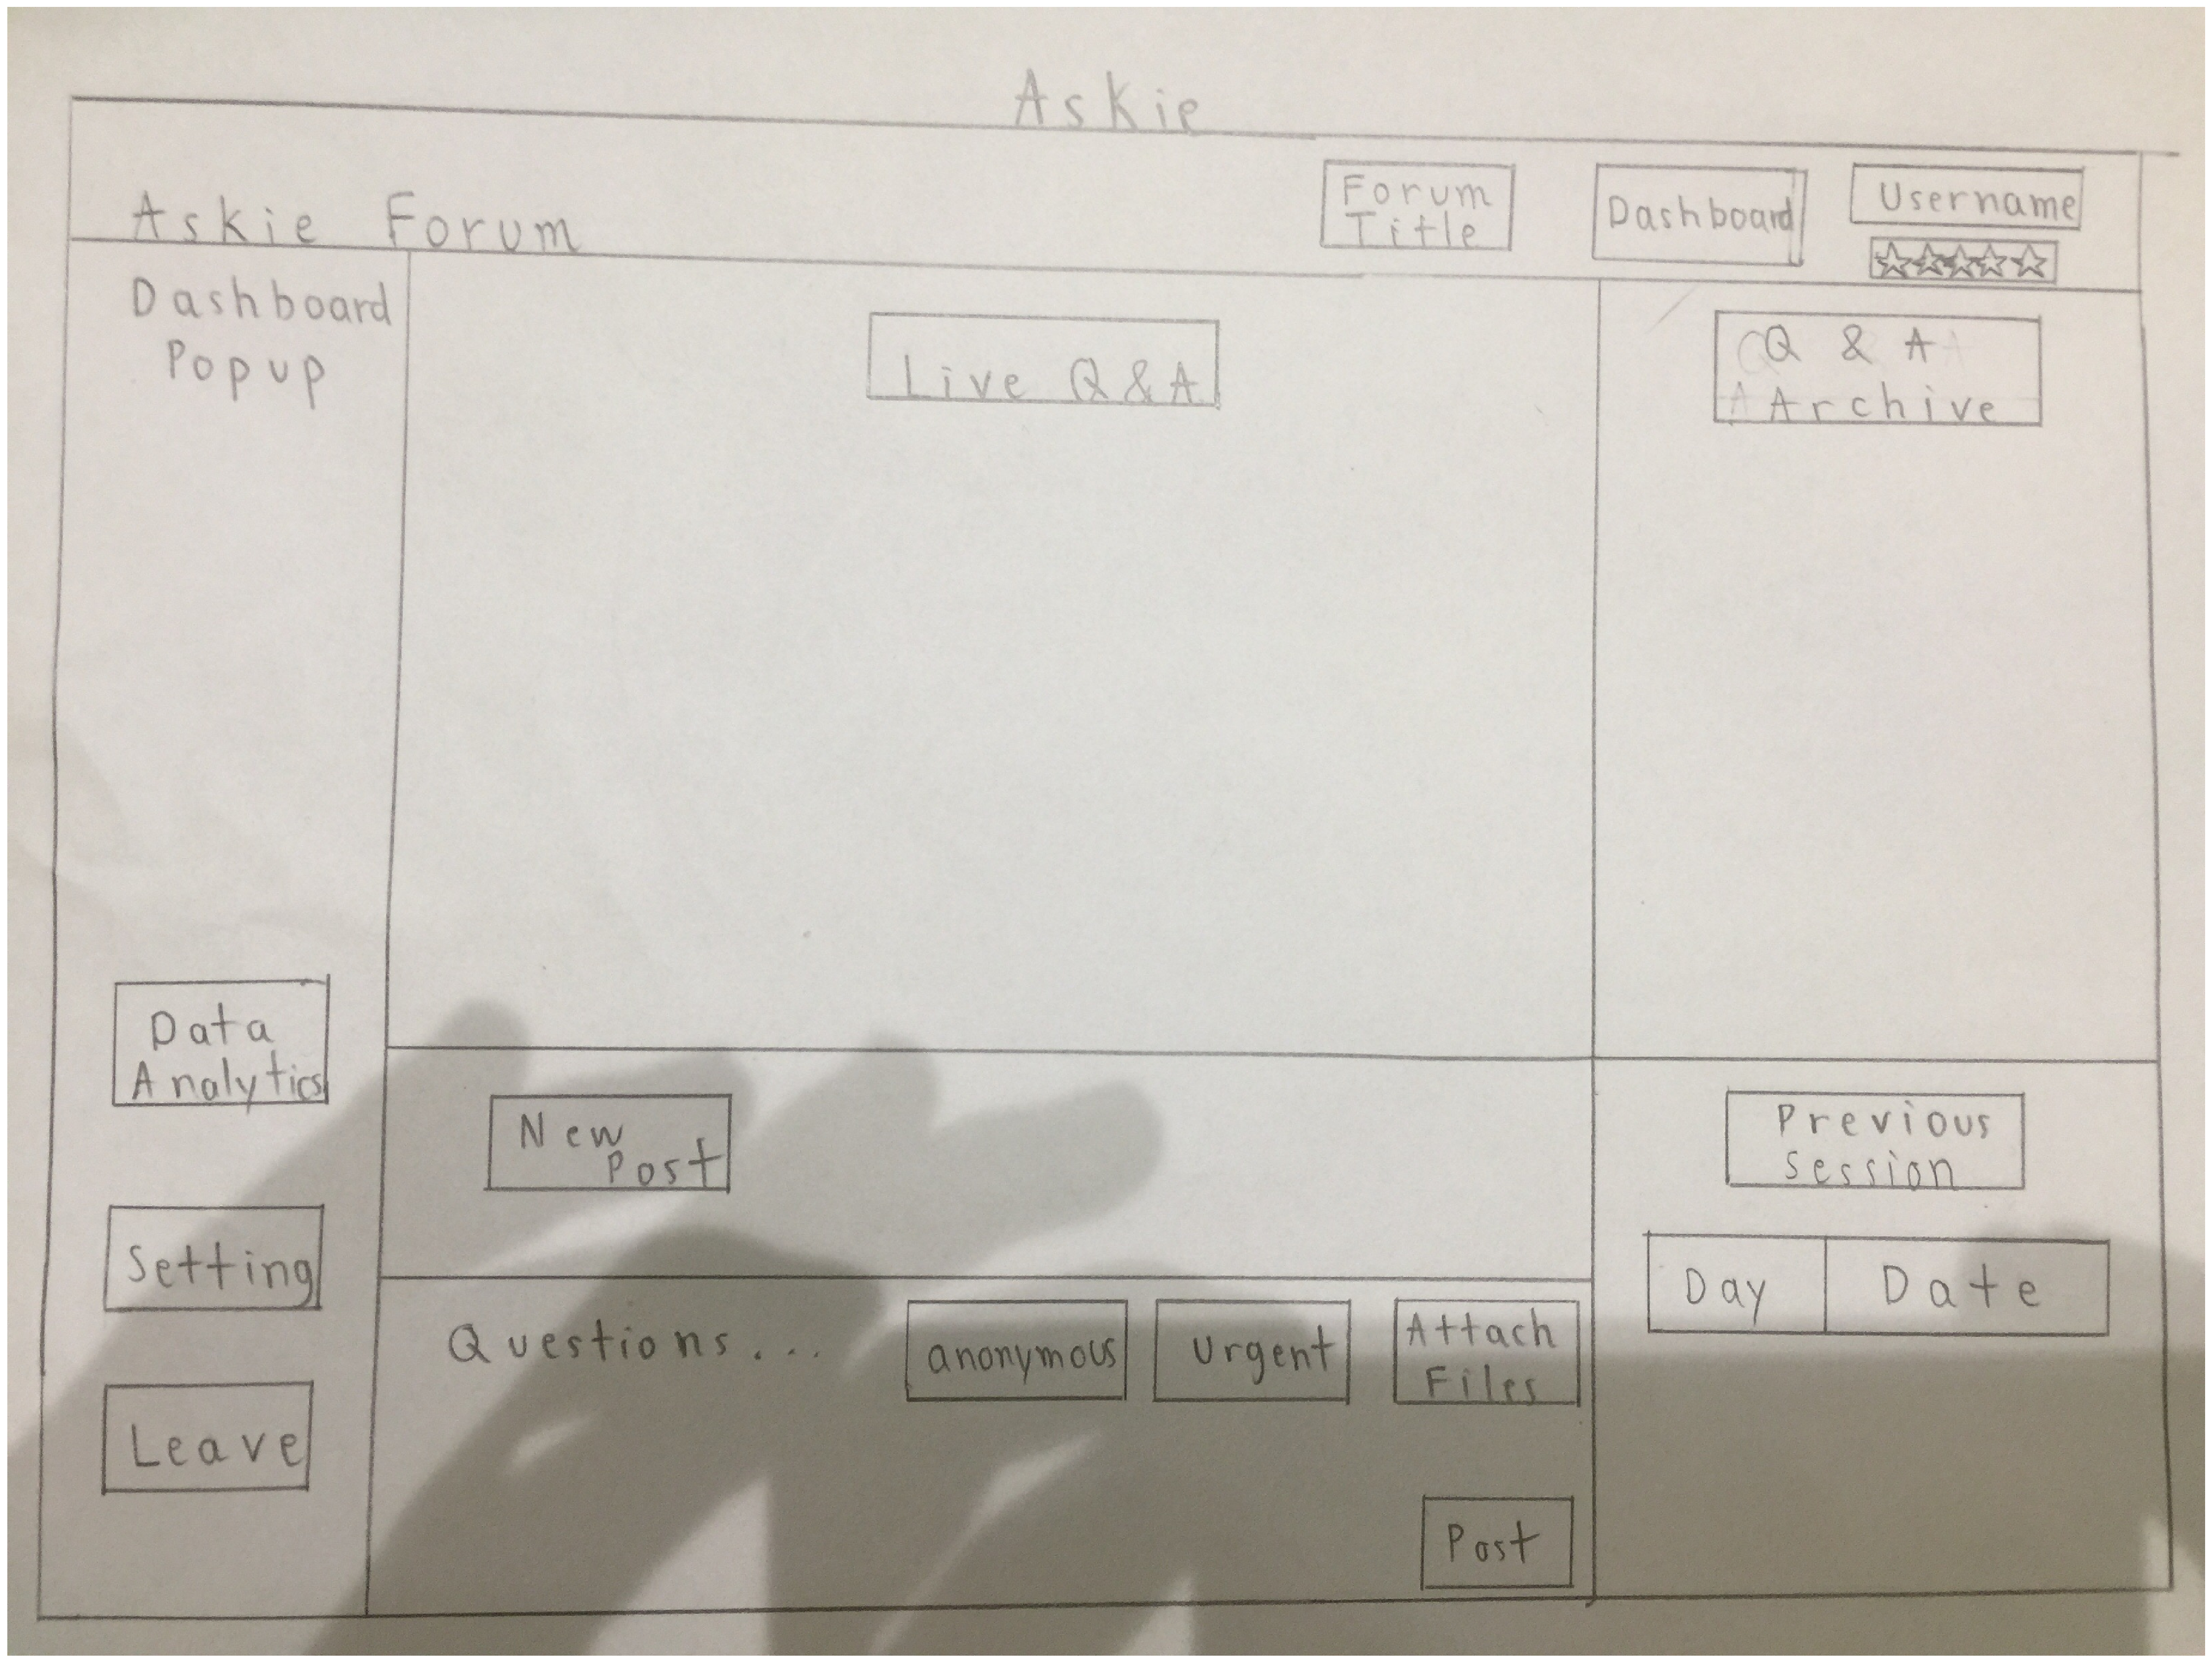
\includegraphics[width=\textwidth]{Assignment_3_UIP1}
\end{flushleft}
\begin{flushleft}
\textbf{Description:} The Askie User Interface represents the screen of users who join a host forum. The top of the interface will display the header bar, which will include the name of our software, "Askie Forum," as well as the name of the forum created by the host. It will also include a dashboard that will allow the user to modify their settings or leave the forum. The last part of the header bar will display the user's name and the rating they've received from other users. The settings option within the dashboard will allow Askie users to set their personal settings, such as how urgent their Urgent Questions might be. A data analytics tab will also be included in the dashboard; its responsibility is to display data about how many questions the user has asked and how many answers they have provided, among other things. The Live Q\&A (Question and Answer) section will let all users within the forum see the questions that have not yet been answered, while the Q\&A Archives will store questions that have been answered over the duration of the session. A similar section called "Previous Session" will be placed at the bottom of the archive section; this section will contain data on the prior session, including questions asked during the previous session of the hosted forum. The last section is the New Post tab, which will allow Askie users to ask questions and tag them as Urgent, Anonymous, etc. It will also allow for users to attach files to their posts. 
\end{flushleft}
\subsection{User Interface for The Host}
\begin{flushleft}
    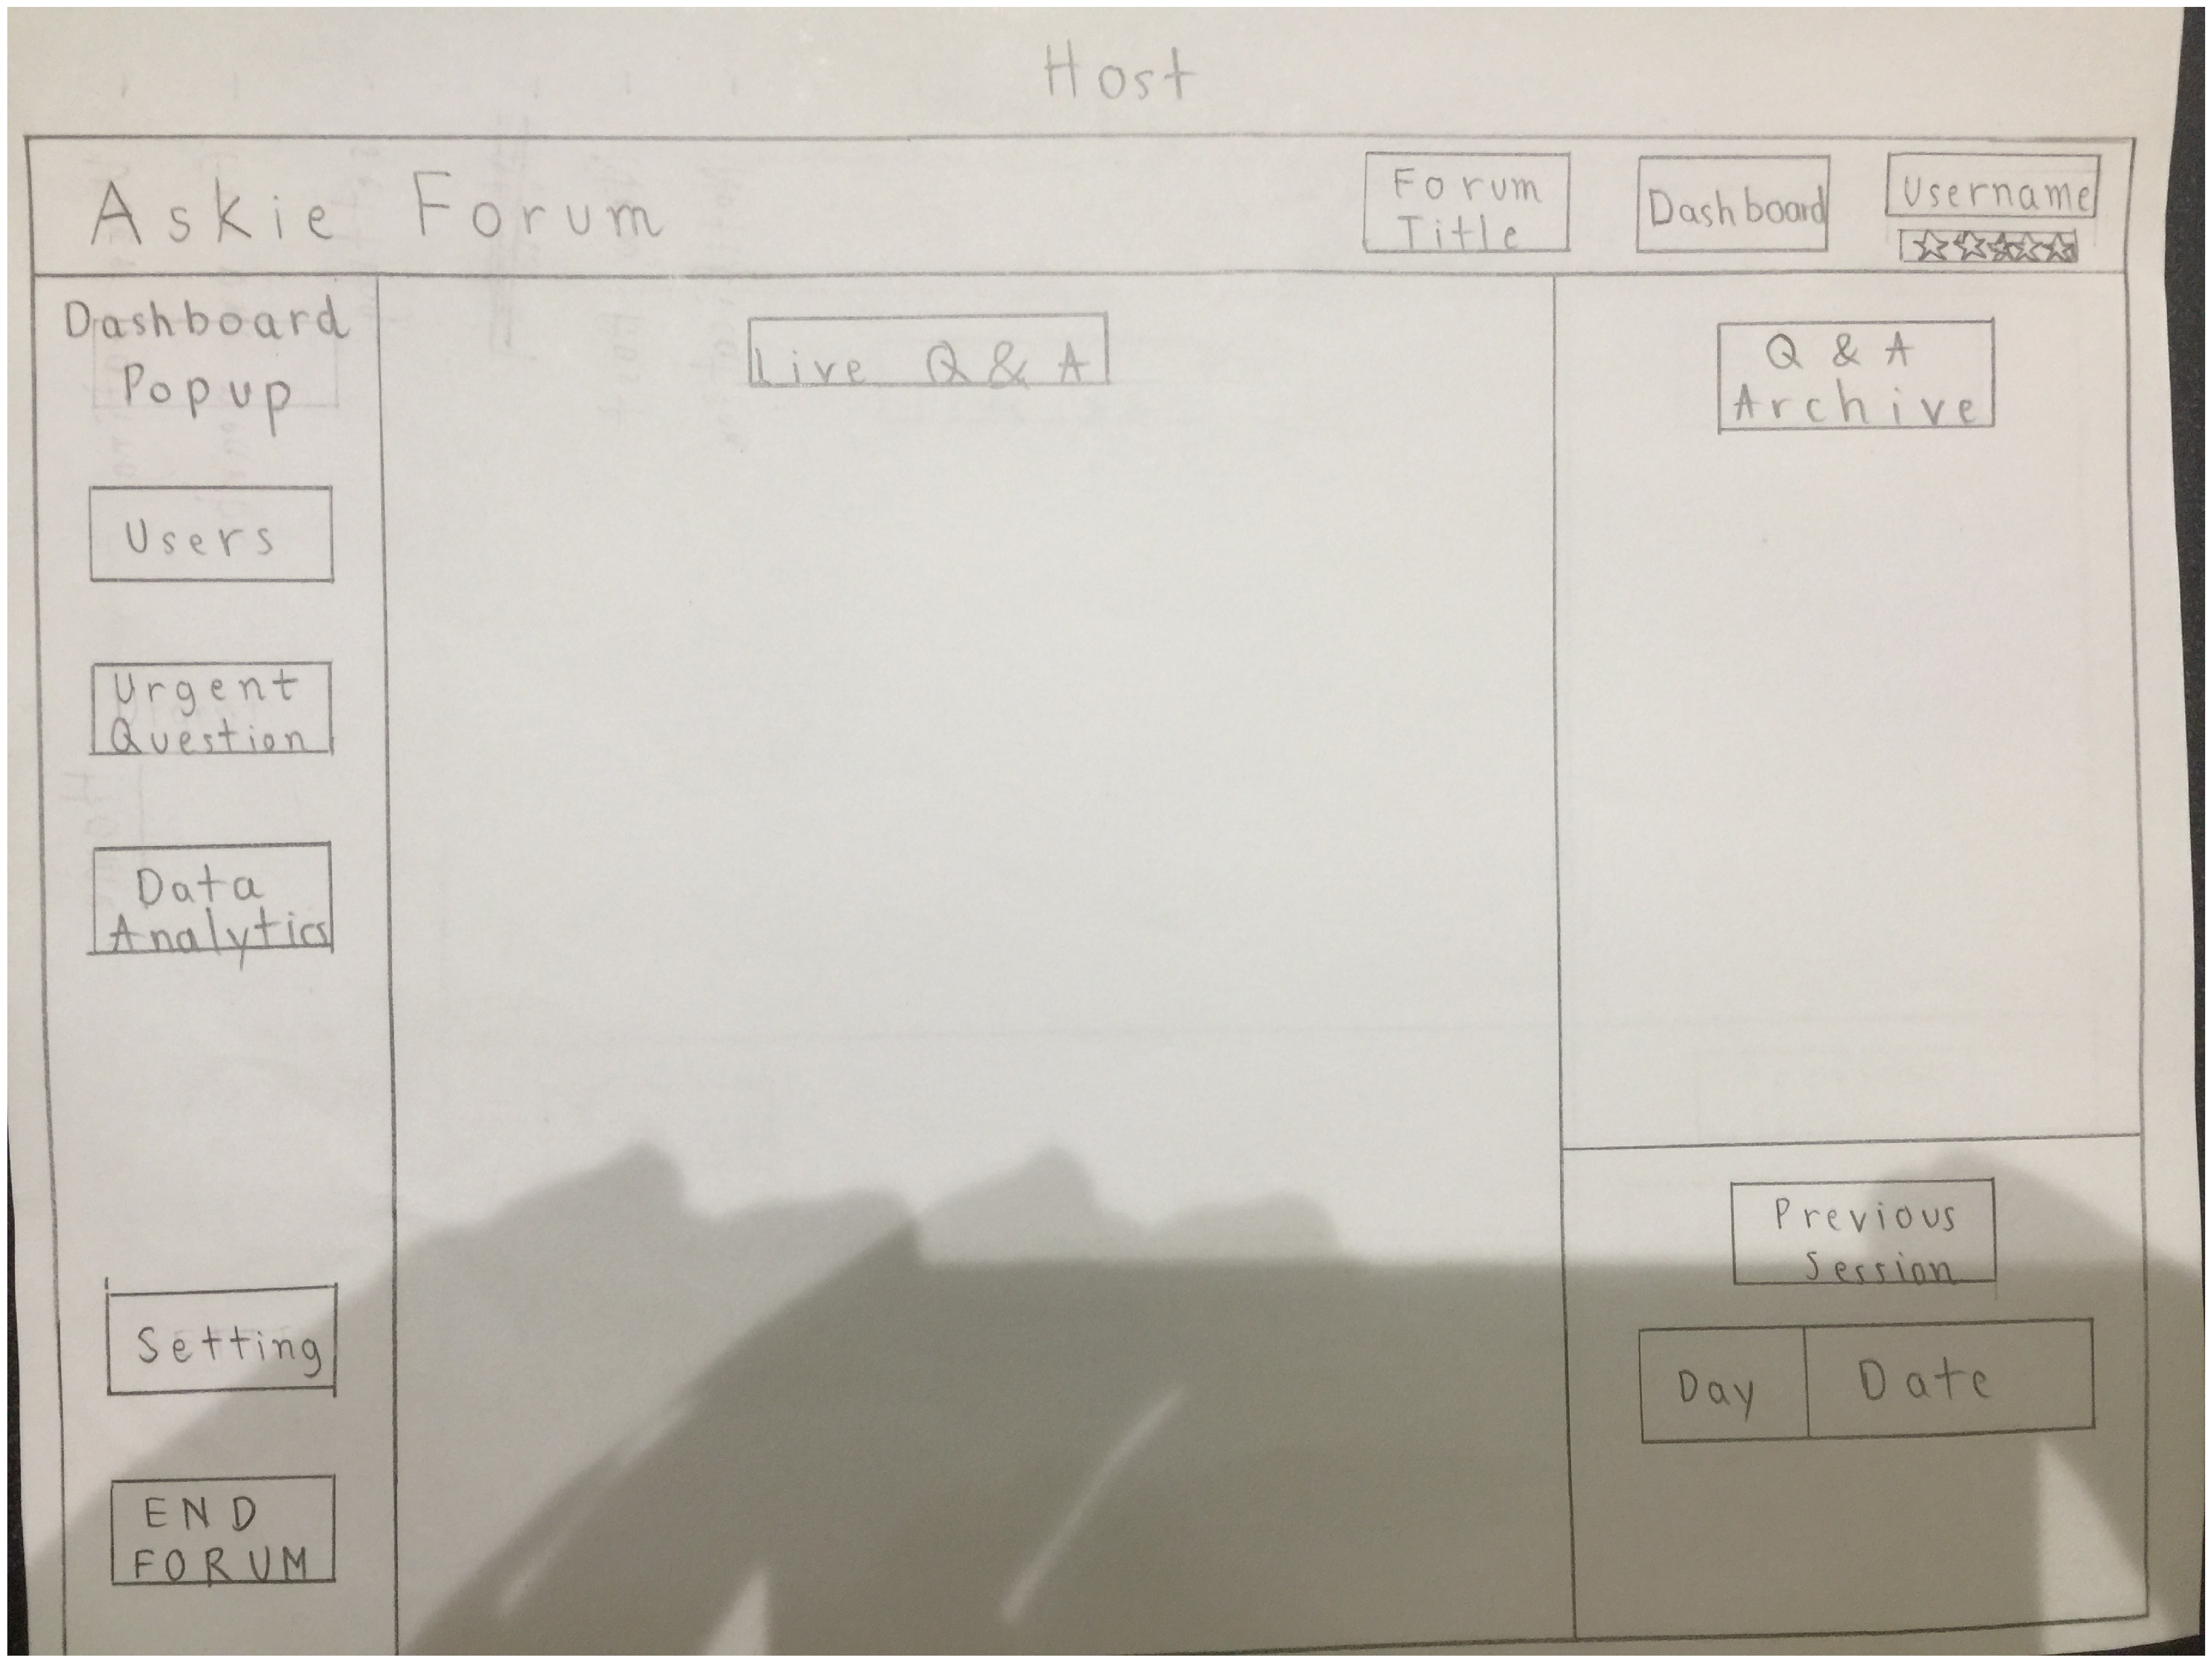
\includegraphics[width=\textwidth]{Assignment_3_UIP2}
\end{flushleft}
\begin{flushleft}
\textbf{Description:} The interface for the host of the forum is quite similar to the UI for Askie users. It also will have a header bar with the name of our software, "Askie Forum," the username and rating of the host, and the title of the Forum. The host's dashboard will have a lot more options than the Askie users', however. The host's dashboard will possess a Users option that will display all users of the forum and an Urgent Question subsection with the listing of all questions that are reserved to be answered by the end of the session. The host's dashboard will also have a data analytics subsection that will calculate the data for users who answer the most and for the users with the highest ratings. The final two subsections are the settings and end forum session sections. Next to the dashboard will be the Live Q\&A section, a segment that displays the questions that are live on the forum. Next to the Live Q\&A will be the Q\&A Archives and Previous Session sections, which will have the same purpose and functionality as their counterparts in the Askie User Interface. 
\end{flushleft}

\subsection{User Interface for Homepage}
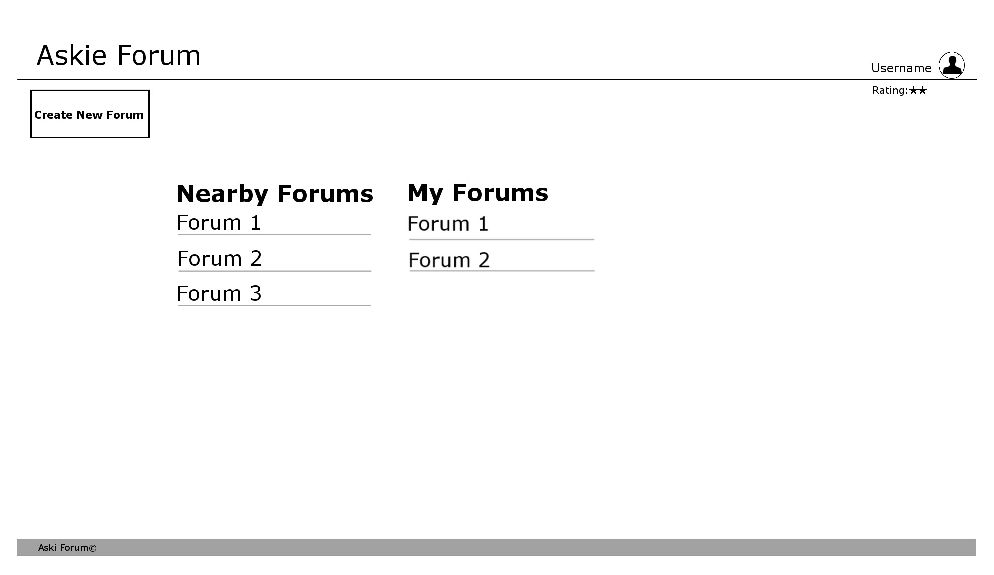
\includegraphics[width=\textwidth]{Askie_Forum_Homepage_UI}
\begin{flushleft}
\textbf{Description:} The homepage is the page that every user will see when they first log in. Only basic information will be displayed here. Users will be able to see their own forums as well as nearby ones. They will also have the option to create a new forum or look at their profile. 
\end{flushleft}

\subsection{User Interface for Welcome Page}
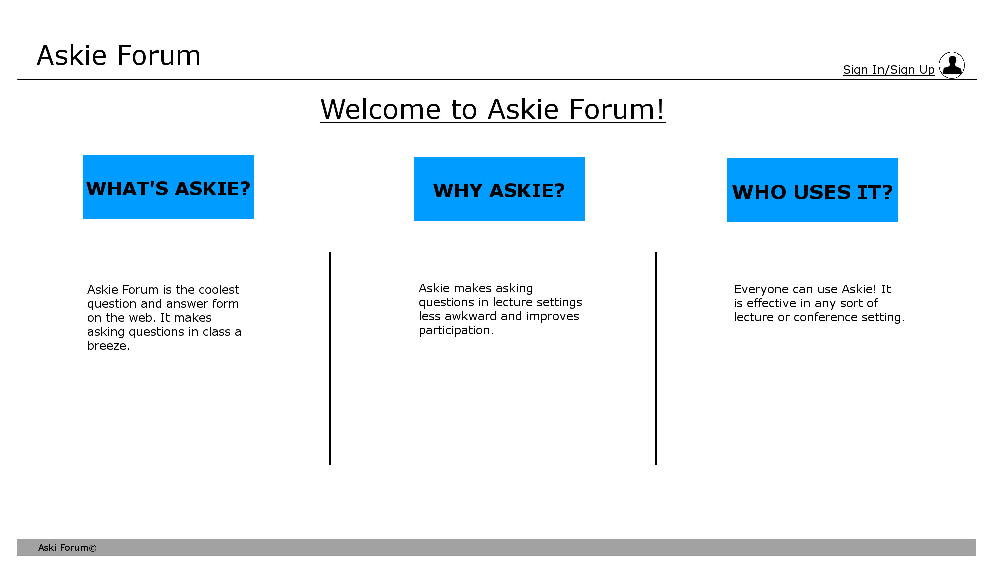
\includegraphics[width=\textwidth]{Askie_Forum_Homepage_UI_logged_out}
\begin{flushleft}
\textbf{Description:} The welcome page is the page that everyone will see before they log into Askie. It will include general information about Askie and will allow the user to either sign in if they've already created an account or sign up if they haven't. Once the user signs in or signs up, they will be taken to the homepage.
\end{flushleft}

\section{Class Diagrams}
\subsection{ERD}
    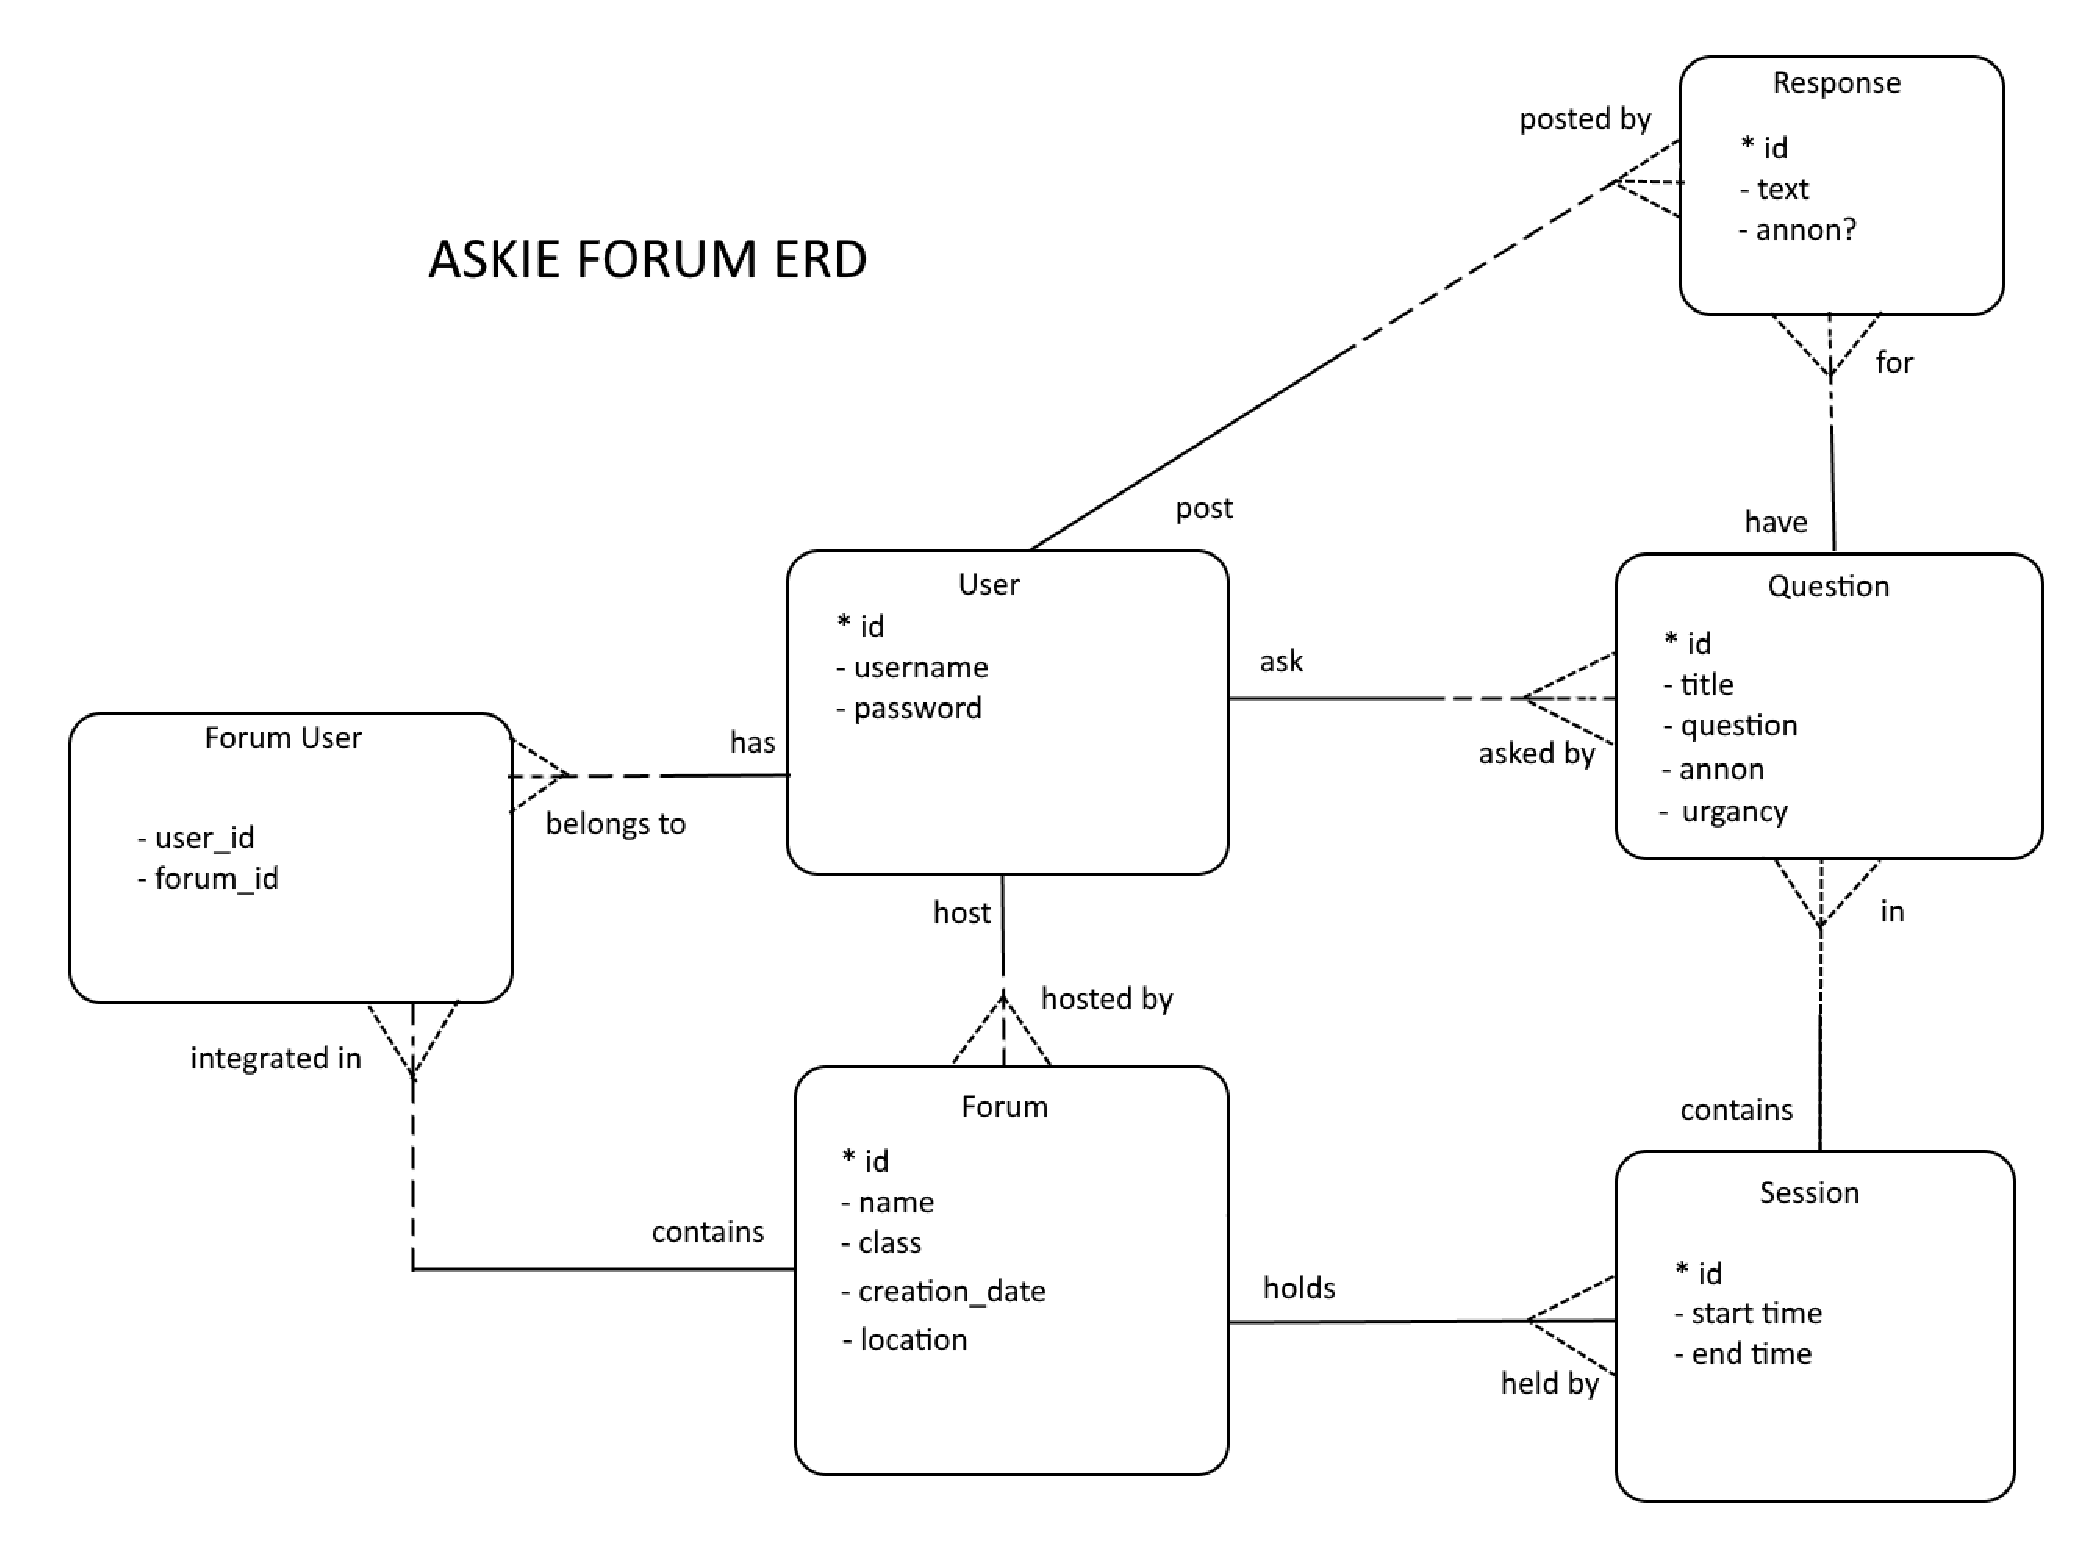
\includegraphics[width=\textwidth]{SoftwareEngineering1_ERD.eps}
\begin{flushleft}
\textbf{Description:} This is the basic Entity Relationship Diagram for our database. It was not a requirement, but it is part of our design stage, and helped with the UML design.
\end{flushleft}
\subsection{UML}
    \includegraphics[width=\textwidth]
{SoftwareEngineering1_UML.eps}
\begin{flushleft}
\textbf{Description:} We used Creately to complete our Askie UML. The User splits into Forum Member and Forum Host as to divide their privileges so that only the host, for example, can create and end forum sessions.
\end{flushleft}



\section{Sequence Diagrams}

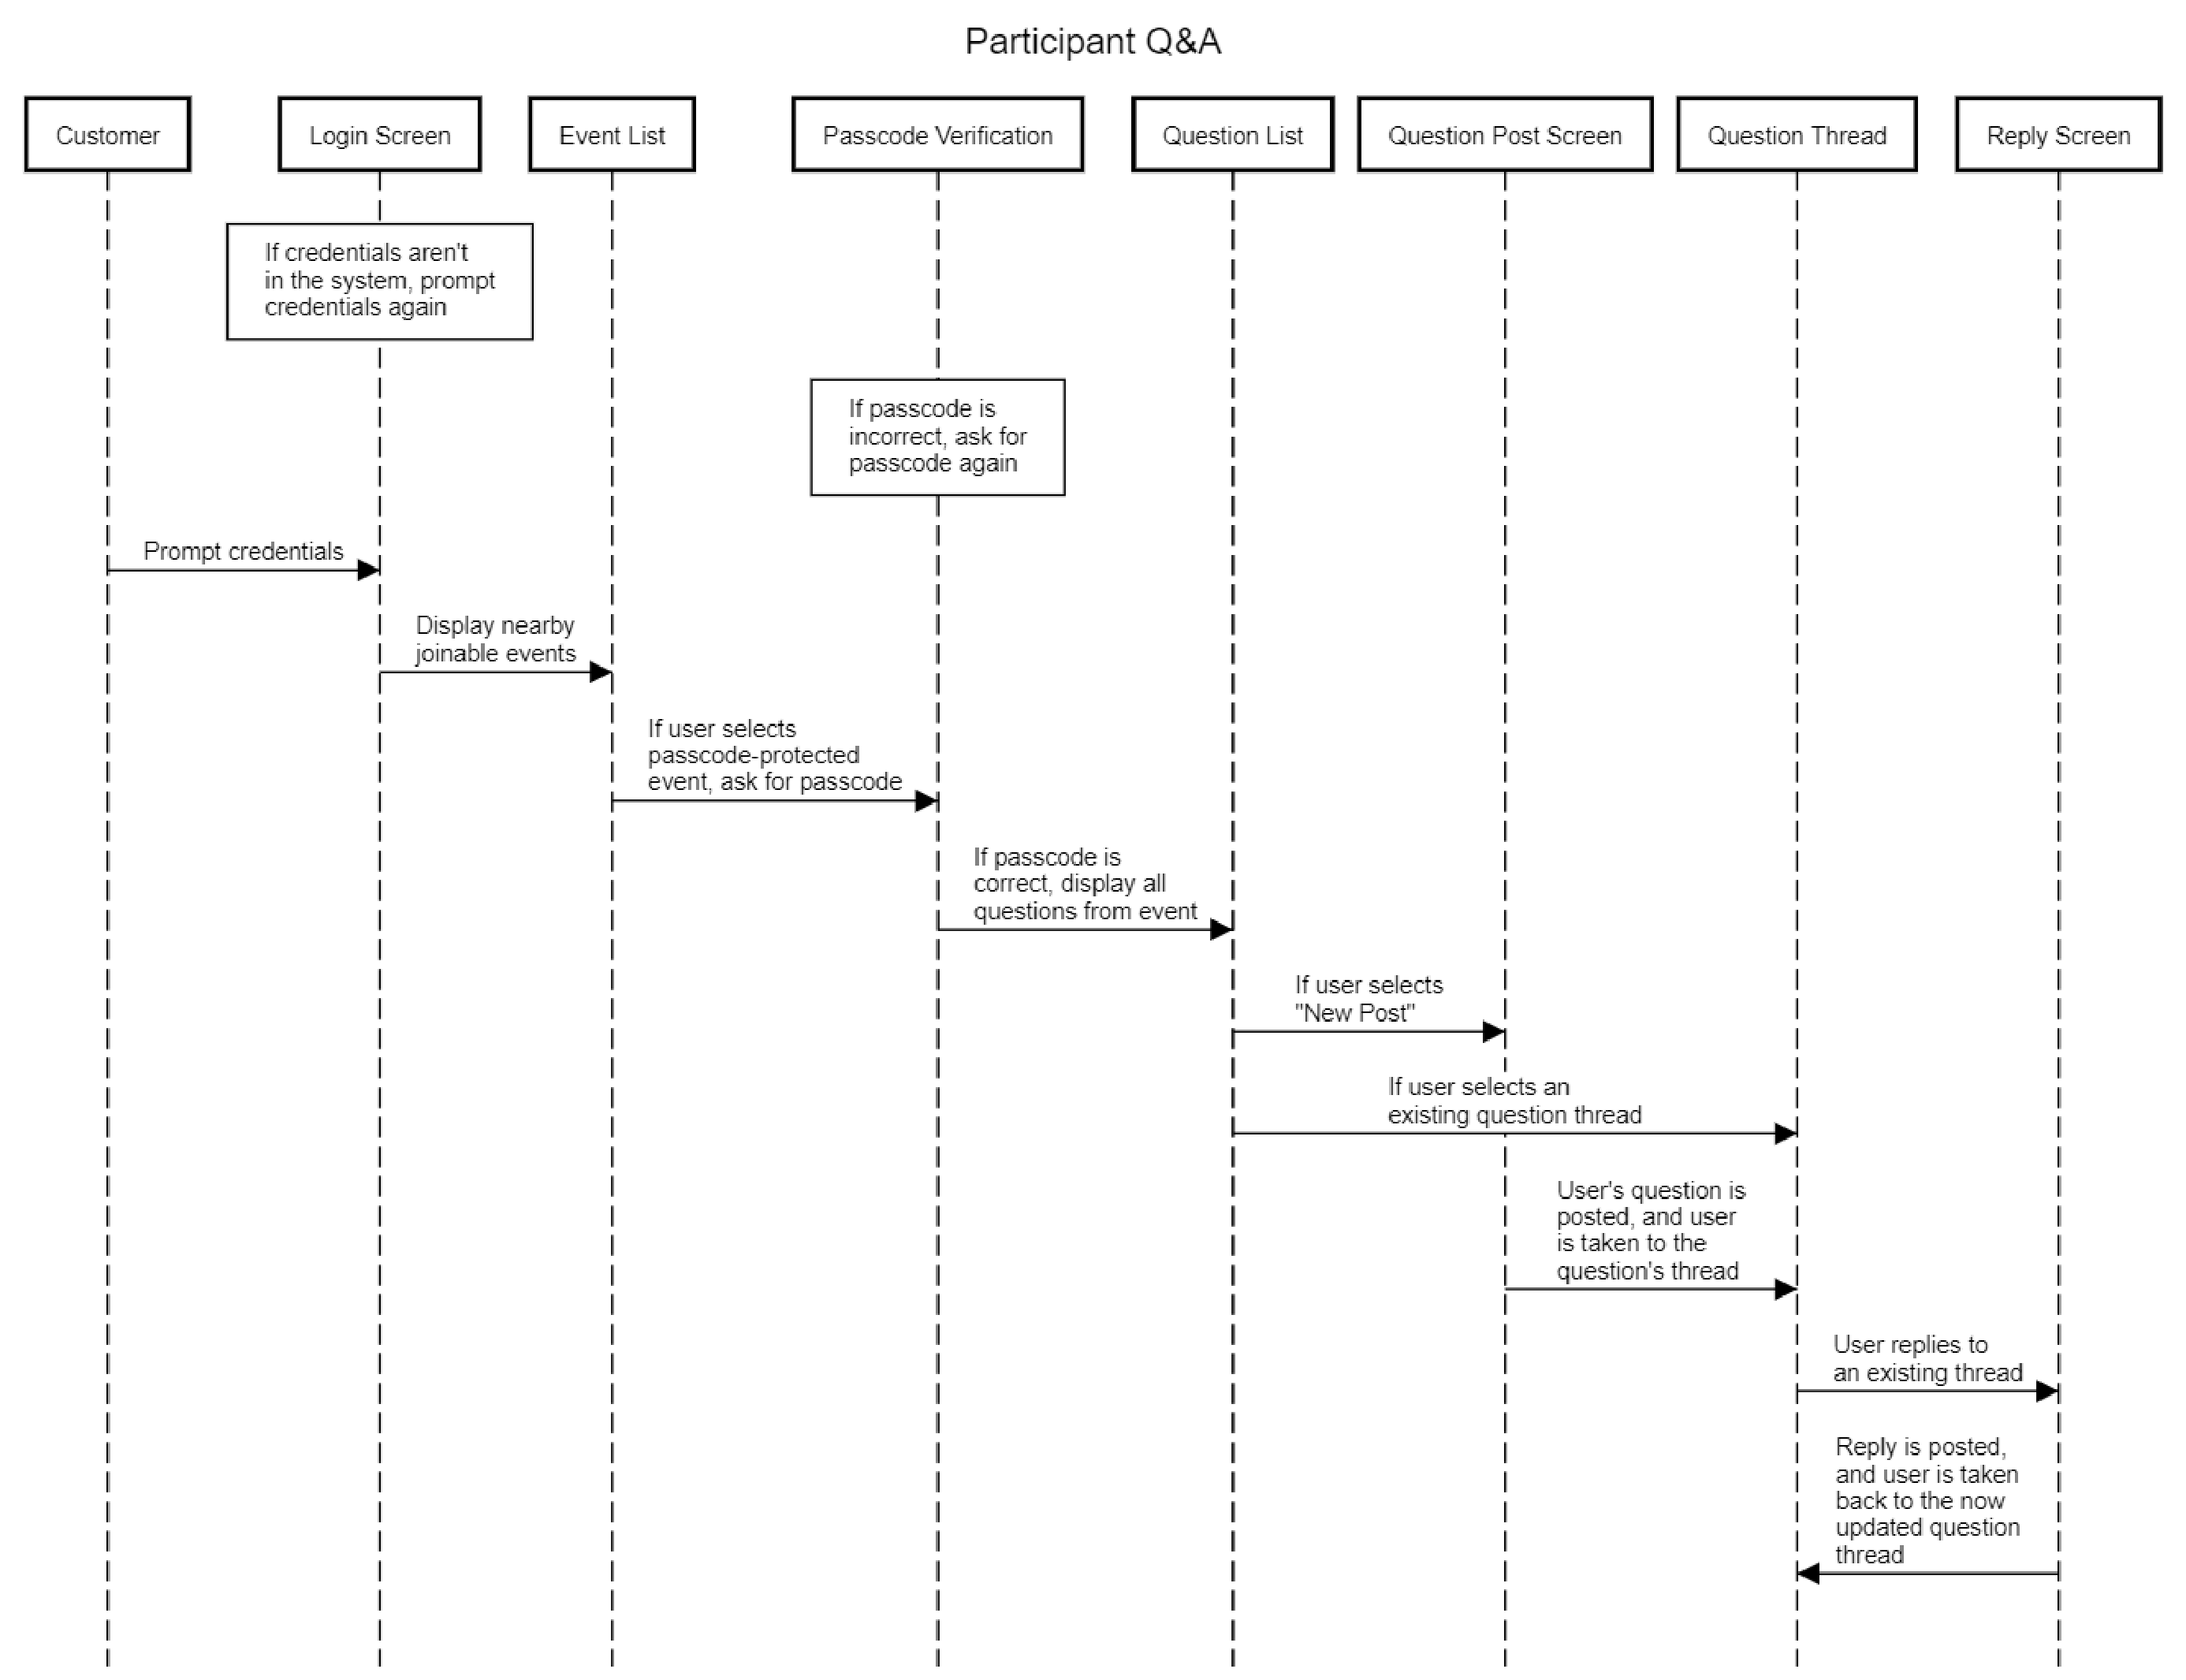
\includegraphics[width=\textwidth]{Participant_QA_Sequence_Diagram_UML.eps}
\textbf{Description:} This sequence diagram details the Participant Question and Answer (Q\&A) use case. The customer - usually either a student or a business meeting participant - logs into their account via a typical login screen. The customer is shown a list of nearby joinable events. Once an event is selected, the user is asked to input a passcode (set by the forum's creator). Inputting an incorrect passcode returns an error message and asks again for the passcode. The correct passcode gives the customer access to the event and brings up a page showing all of the event's questions. From there, the user has two primary options: they may post a new question or select an existing question. Opting to post a new question brings up the question post screen. Once the question is written and posted, the user is directed to the thread of the question they just posted. If the user had instead chosen to view an existing thread rather than post a new question, they would have been directed to the selected question thread. When the user is on an existing thread (whether or not they created the question), they will be given the option to reply to the thread using the reply screen. After the reply is posted, they will be directed back to the now updated question thread.

\includegraphics[width=\textwidth]{Participation_Required_Sequence_Diagram_UML.eps}
\textbf{Description:} This sequence diagram details the Participation Required use case, and takes into account the potential actions of two possible actors: an instructor and a student. This use case can also be used for a business setting - in that case, simply change "instructor" and "student" to appropriate titles (e.g. "meeting leader" and "participant").

\begin{flushleft}
Instructor: The instructor logs in using an instructor account, enabling them to create events. They are then given the option to join an existing event or create a new one. Joining an existing event for which the instructor does not have instructor privileges effectively renders them a student, as far as this use case is concerned. Choosing instead to create an event brings up the event creator screen, which the instructor may use to customize certain aspects of the event (such as whether or not students can post their own questions in the forum). After the event is created, the instructor is brought to the question list, where they may post questions for students to answer. This is performed using the question post screen.
\end{flushleft}

\begin{flushleft}
Student: The student logs in using a student account. They are shown a list of nearby joinable events. Once an event is selected, the user is asked to input a passcode (set by the forum's creator). Inputting an incorrect passcode returns an error message and asks again for the passcode. The correct passcode gives the customer access to the event and brings up a page showing all of the event's questions. As participation is required in this use case, the student must post an answer to all questions that their instructor is requiring them to answer. When they select a question, the student is given the option to post a response to the question, which will be viewable only by the instructor and the student who authored the post. Unless the instructor explicitly allows it, students may not view posts created by other students in any given question thread. This format is useful for things like in-class activities and quizzes.
\end{flushleft}


\includegraphics[width=\textwidth]{Live_Q_A_1_.eps}
\textbf{Description:} This sequence diagram details the Live Q/A use case, and takes into account the potential actions of two possible actors: an instructor and a student. Here it is assumed that the instructor (or relevant event leader) has the Askie forum open, and is waiting for questions from students/participants.

\begin{flushleft}
Instructor: The instructor logs in using an instructor account, enabling them to create events. They are then given the option to join an existing event or create a new one. As above, joining an existing event for which the instructor does not have instructor privileges effectively renders them a student. Choosing instead to create an event brings up the event creator screen, where instructors can customize certain aspects of the event (such as whether or not instructors/moderators get notified of new questions). After the event is created, the instructor is brought to the question list. For this use case it is generally assumed the instructor isn't answering questions via text. Instead, as new questions get posted, the instructor is notified so as to have the ability to work the answers seamlessly into his or her presentation. Other students still have the ability to answer as well.
\end{flushleft}

\begin{flushleft}
Student: The student logs in using a student account. They are shown a list of nearby joinable events. Once an event is selected, the user is asked to input a passcode (set by the forum's creator). Inputting an incorrect passcode returns an error message and asks again for the passcode. The correct passcode gives the customer access to the event and brings up a page showing all of the event's questions. From here, it is assumed that the student will primarily be asking new questions, however they still have the ability to answer the questions of other students as well. For this use case, we also assume that the instructors/moderators are getting notified of new questions. As it it likely that a question might not get answered in textual form, a moderator may have to manually delete the question after it is answered in person.
\end{flushleft}


\section{Meeting Report}
\begin{flushleft}
The most productive processes of the week were the design of the user interface for Askie users and hosts, and the design of the home screen of Askie Forum. We have validated the purpose of our software with the survey. The UI design will allow us to take a big step toward the implementation of the software. Having a design will help make creating the application a lot quicker since we know exactly what it will look like. The design will also give us a clear indicator of what each section of the screen will include. What we hope to accomplish this coming week is the completion of all attributes and capabilities of the home page. The complete homepage will allow user to create an account, which will then allow them to host a forum or join a nearby forum. To recap, our goal this coming week is to start working on the outline of the home page, and then provide a database to contain user information, such as usernames. This week's tasks were divided as follows: Joshua Bell, Andrew Morill and Danh Nguyen created the User Interface Prototypes; Andrew Morill created the Class Diagrams; Danh Nguyen created the Meeting Report; and Cameron Kocher and Nicholas Newell created the Sequence Diagrams and descriptions.
\end{flushleft}

\section{Reference}
\begin{center}
[1] \url{https://docs.google.com/forms/d/1Iy_wi3jled_O1cKcYa2V-x7rIAkfquGEKGC7UuGZPaM/edit}


[2] 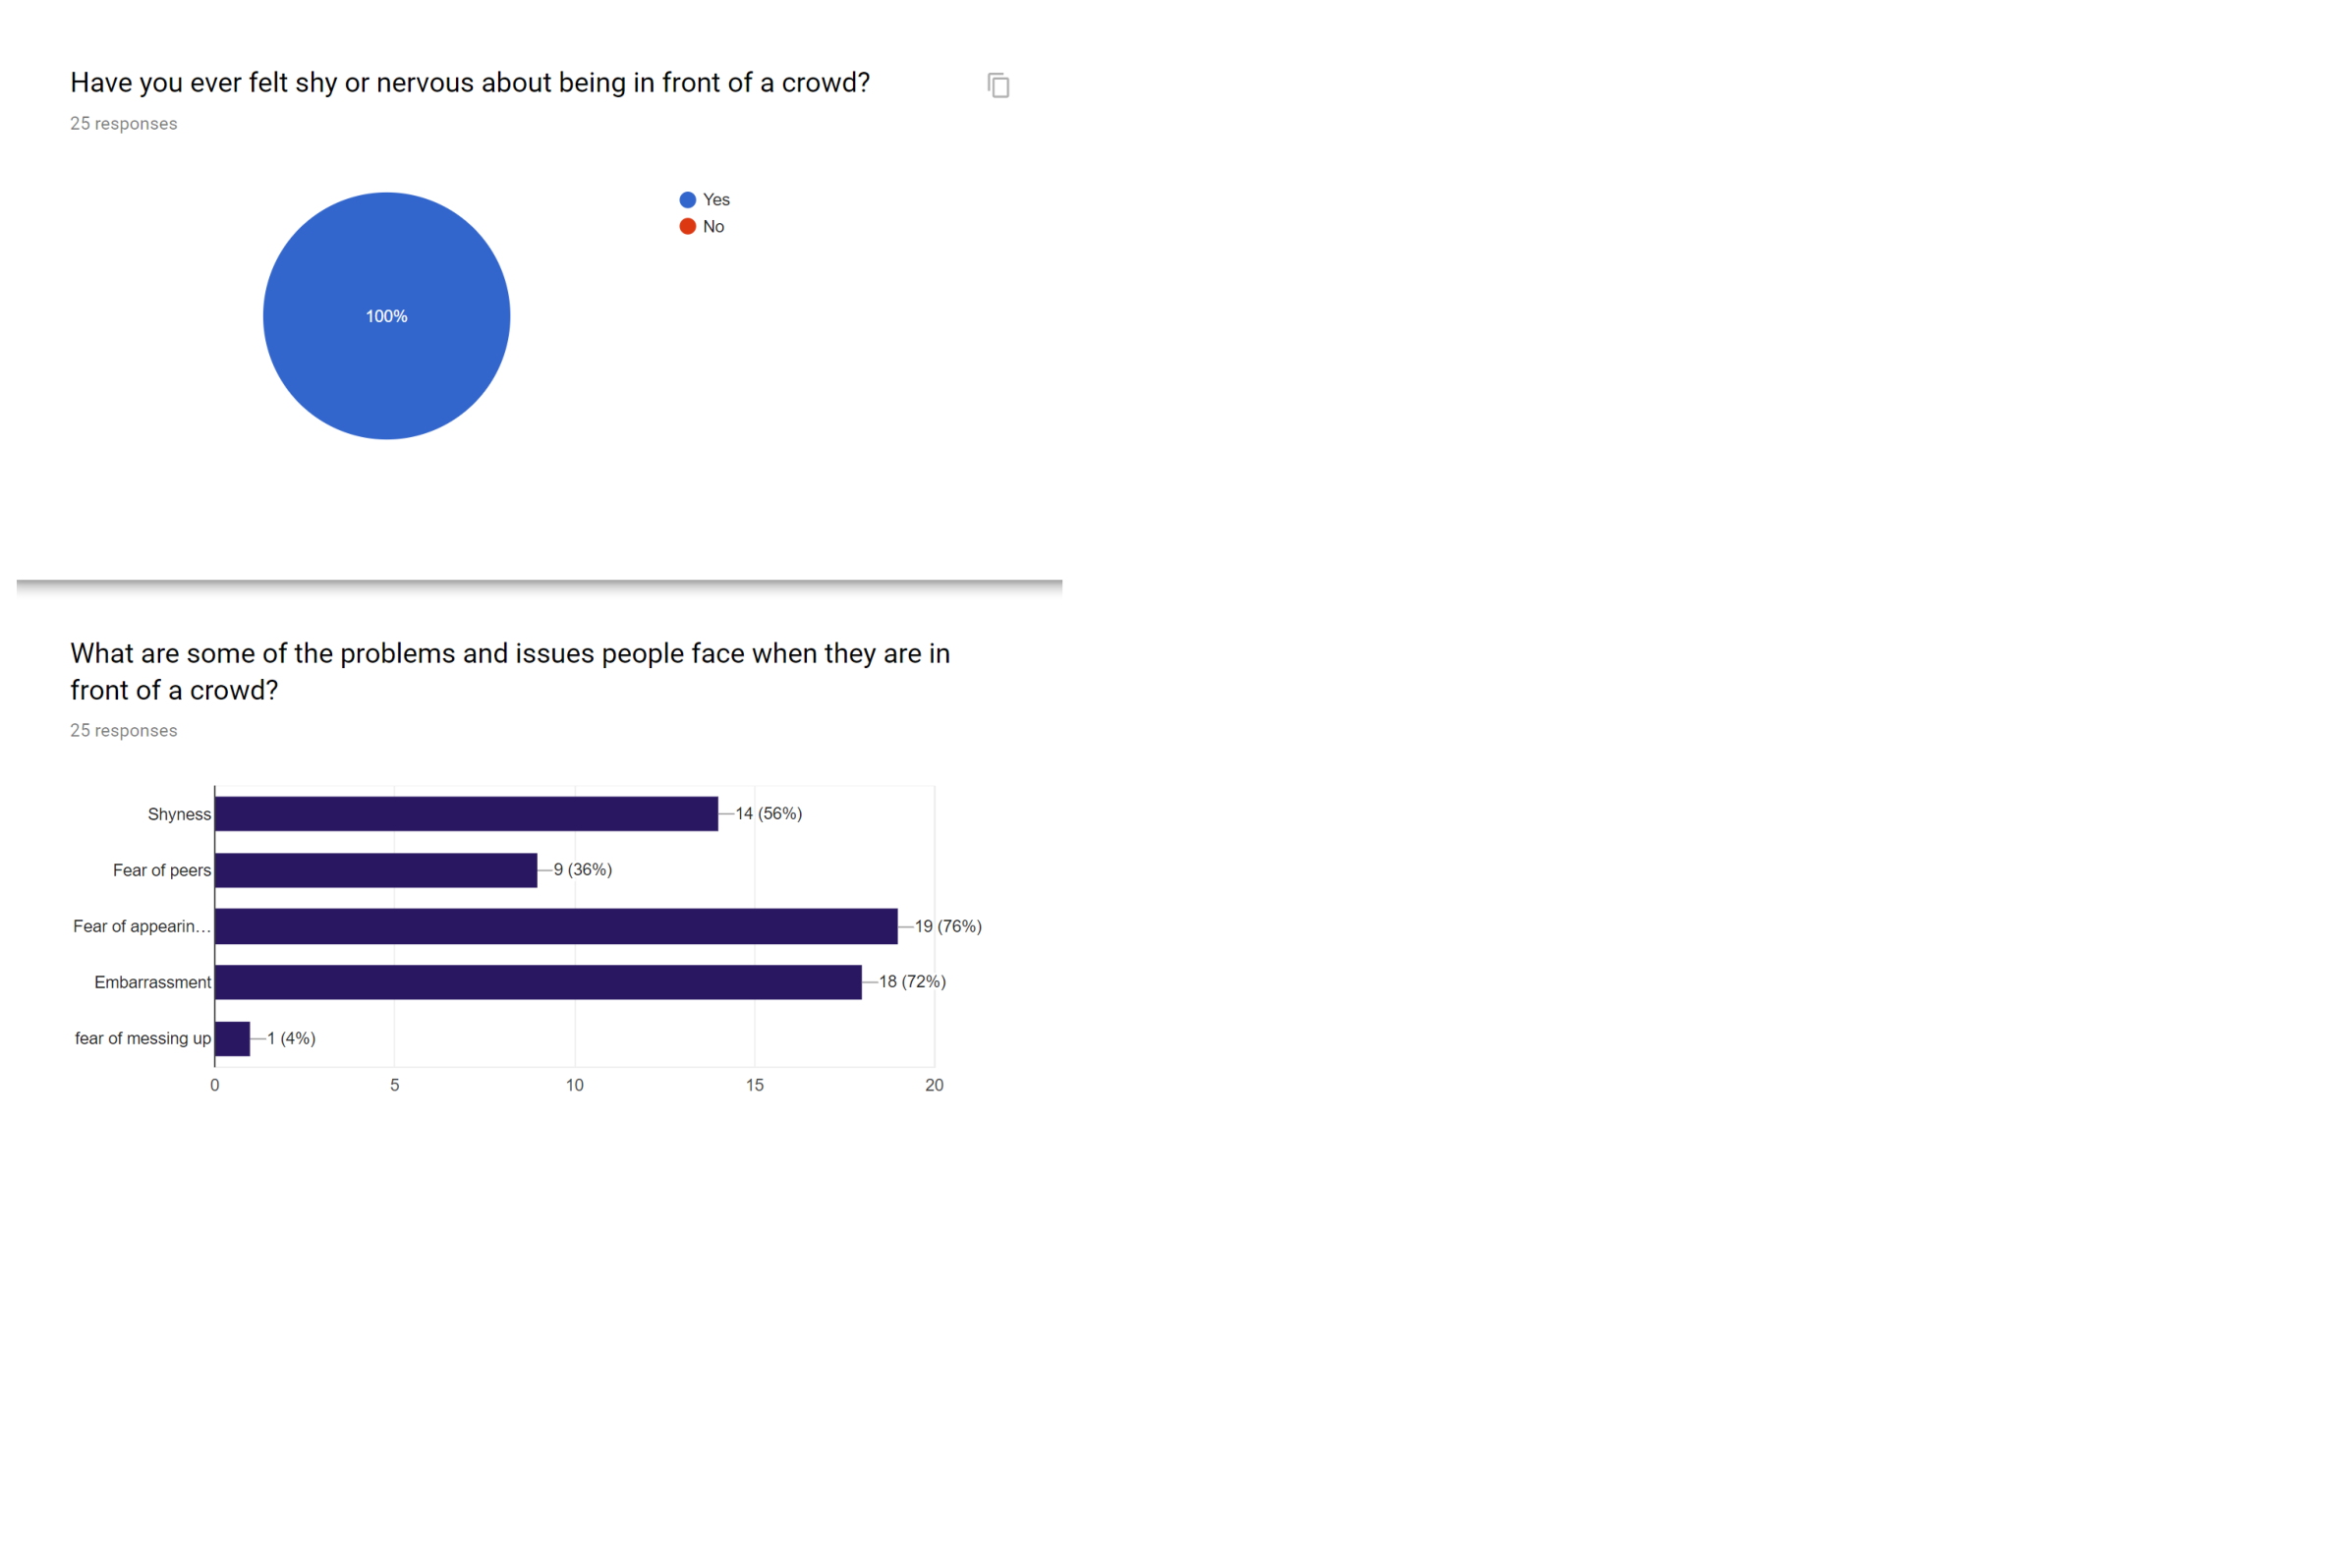
\includegraphics[width=\textwidth]{Assignments_reference_2}


[3] 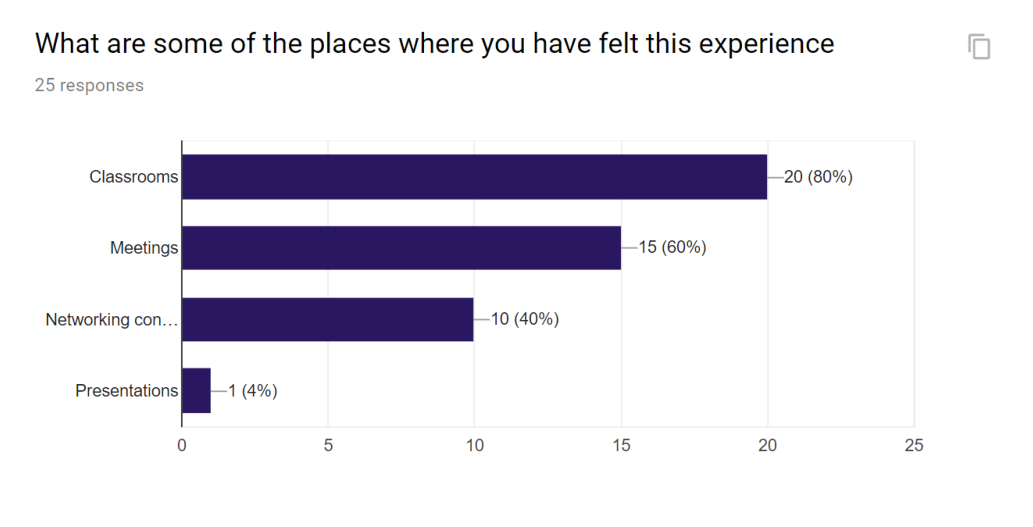
\includegraphics[width=\textwidth]{Assignments_reference_3}


[4] 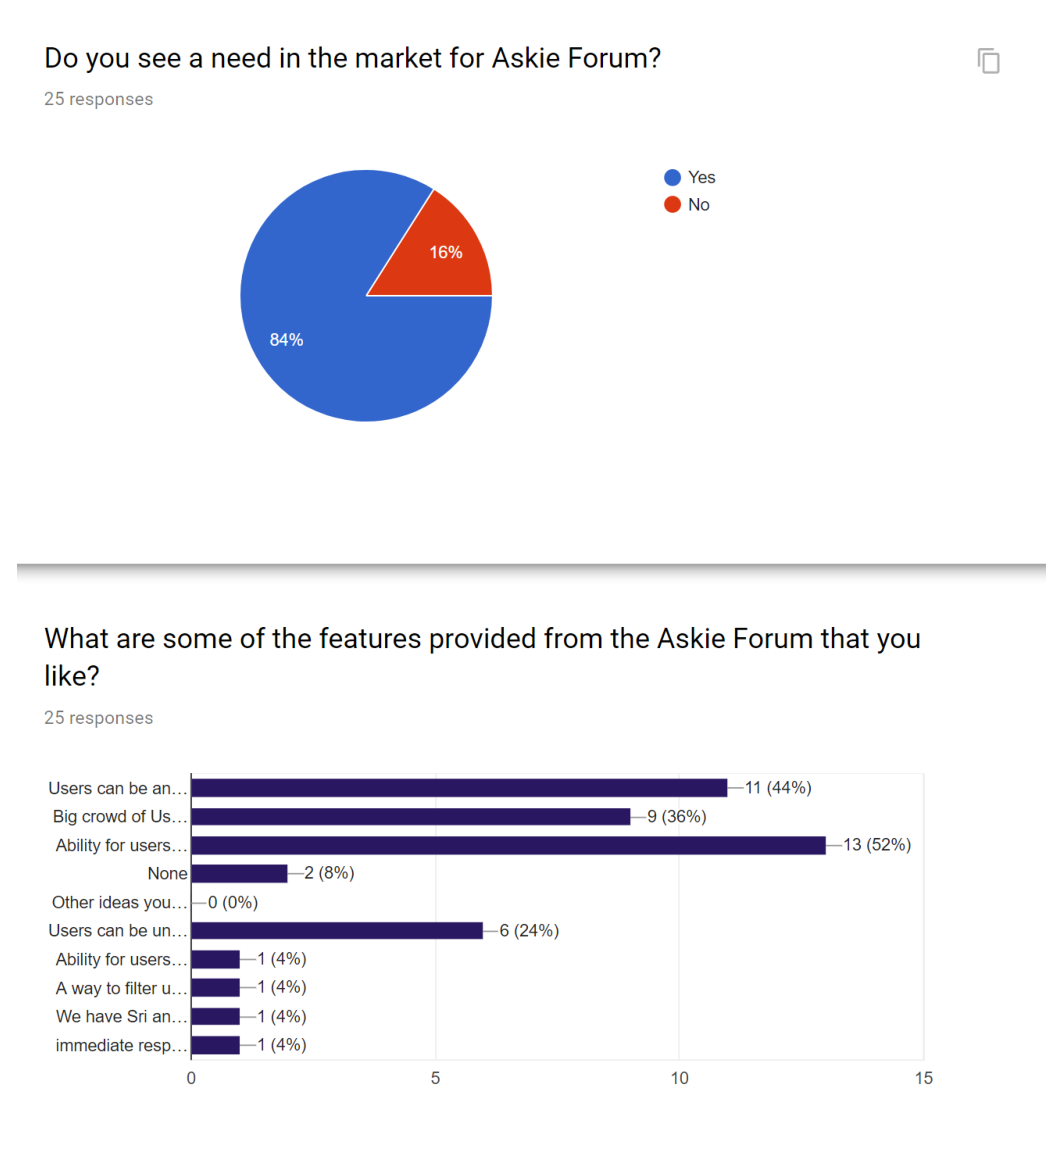
\includegraphics[width=\textwidth]{Assignments_reference_4}


[5] 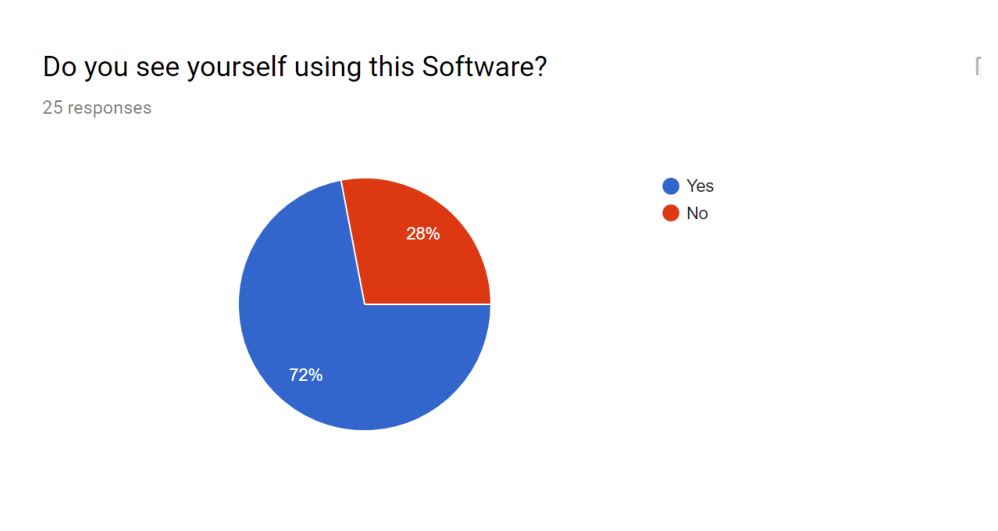
\includegraphics[width=\textwidth]{Assignments_reference_5}
\end{center}


\end{document}
